\chapter{Inferenza della struttura}
\section{Analisi delle tecniche utilizzate}
\label{sec:misure}
Il nostro obiettivo principale è quello di verificare se sia possibile apprendere la struttura della rete a partire da un dataset contenente i dati di $10000$ pazienti con la sindrome del \textit{Blue Baby}. Al fine di fare ciò, sono state considerate due differenti approcci, ovvero la tecnica \texttt{Hill Climb} e la tecnica \texttt{Tabù Search}. Entrambe le tecniche sono basate su un processo meta-euristico di ottimizzazione di una funzione di \textit{score}. Documentandoci sulle due tecniche prese in esame, ed effettuando alcuni test preliminari, abbiamo notato come le performance della ricerca Tabù siano superiori a quelle della prima tecnica citata, in quanto Tabù evita di cadere e rimanere in minimi locali.\\
\begin{table}[t!]
	\centering
	\caption{Differenti funzioni di \textit{score} a confronto. La colonna \textit{Archi paper} mostra il numero di archi presenti nella rete proposta dal paper ma non presente nel modello generato. Viceversa, l'ultima colonna indica il numero di archi presenti nel modello appreso ma non presenti nella rete dell'articolo.}
	\begin{tabular}{|c|c|c|c|c|}
		\hline 
		Funzione & Archi generati  & Archi comuni & Archi paper & Archi appreso \\ 
		\hline 
		aic & 32 & 24 & 1 & 8 \\ 
		\hline 
		bic & 26 & 18 & 7 & 8 \\ 
		\hline 
		bde & 26 & 21 & 4 & 5 \\ 
		\hline 
		bds & 26 & 18 & 7 & 8 \\ 
		\hline 
		mbde & 26 & 21 & 4 & 5 \\ 
		\hline 
		bdla & 26 & 21 & 4 & 5 \\ 
		\hline 
		k2 & 25 & 24 & 1 & 1 \\ 
		\hline 
	\end{tabular} 
	\label{tab:score}
\end{table}
Abbiamo quindi approfondito le possibili funzioni di \textit{score} disponibili per la ricerca Tabù, confrontando la rete prodotta con quella fornita dal \textit{paper} di riferimento. I risultati ottenuti, proposti in Tabella \ref{tab:score}, mostrano come molte misure ottengano performance simili, mentre quella che si distingue dalle altre risulta essere la funzione \texttt{k2}, che permette di stimare correttamente il numero di archi, inserendo un solo arco in posizione non concorde con la rete fornita dal \textit{paper}.

La Figura \ref{fig:inducedstructure} mostra la rappresentazione prodotta dall'algoritmo \texttt{Tabù Search} con la funzione di \textit{score} \texttt{k2}; confrontando questa struttura con quella proposta in Figura \ref{fig:paperstructure}, notiamo come l'unico arco differente sia quello che collega i nodi \textit{Age} e \textit{Sick}.

\begin{figure}
	\centering
	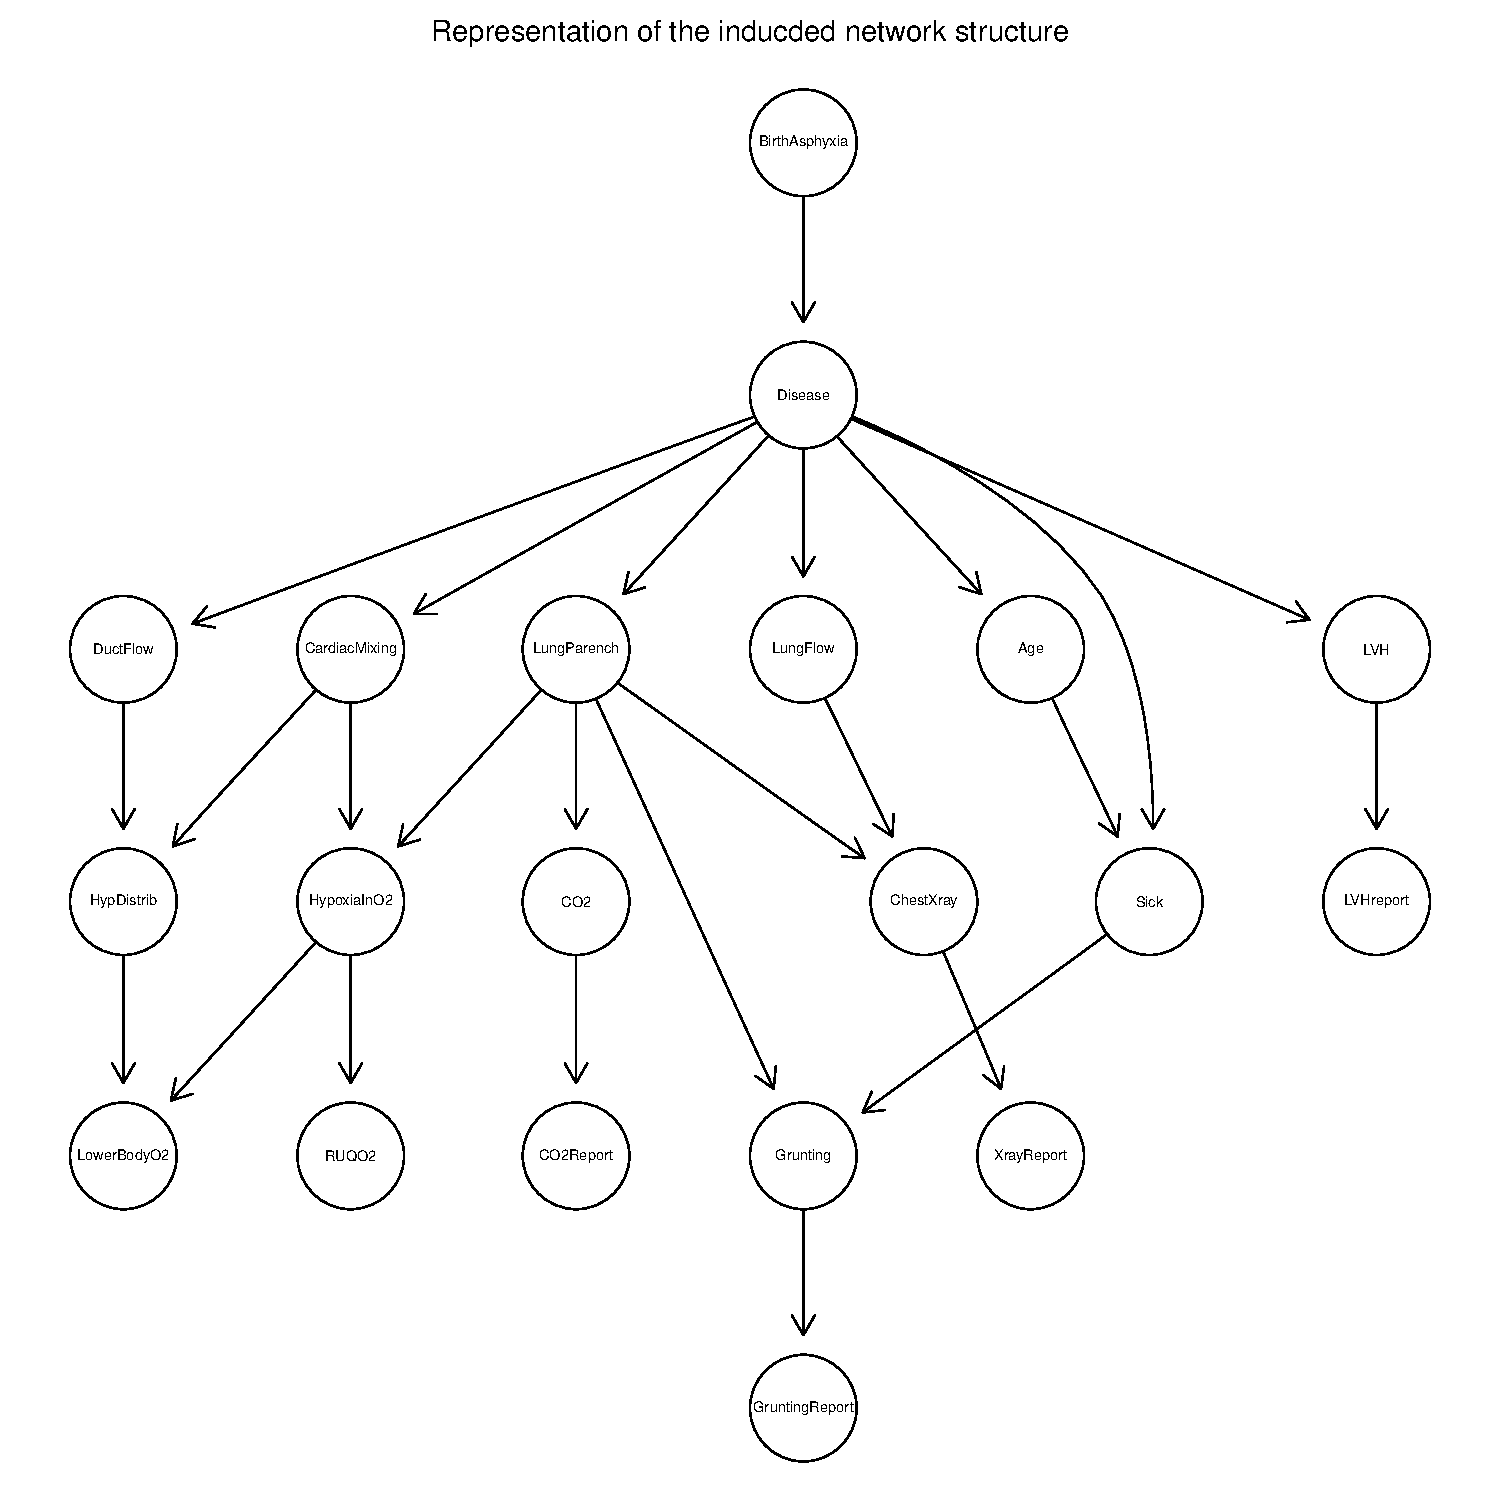
\includegraphics[width=.9\linewidth]{images/induced_structure}
	\caption{Rappresentazione della struttura appresa con la ricerca di Tabù e la funzione di \textit{score} \texttt{k2}}
	\label{fig:inducedstructure}
\end{figure}

\newpage
\section{Misure di performance delle reti}
\label{sec:performance}
Una volta indotta la struttura della rete con il metodo illustrato nella Sezione \ref{sec:misure}, abbiamo deciso di valutare le capacità predittive della reti proposte per quanto riguarda la predizione della variabile \textit{Disease}. Per fare ciò, abbiamo deciso di effettuare un'operazione di \textit{10-times 10-fold coross validation}, al fine di garantire la significatività statistica dei risultati ottenuti. In ogni fold, per le due reti vengono stimate le CPT di ogni nodo utilizzando il $90\%$ del dataset; viene poi utilizzata la tecnica \textit{likelihood weighting}, generando 500 sample per ogni nuova osservazione, per determinare il valore del nodo \textit{Disease} associato ad una particolare istanza.

Le performance ottenute, riportate nelle Figure \ref{fig:paperperformance} e \ref{fig:inducedperformance}, calcolate come la media delle dieci ripetizioni del processo di \textit{cross validation}, risultano essere molto simili. Al fine di indagare se le performance dei due modelli proposti fossero statisticamente differenti, sono stati eseguiti dei test di significatività \textit{t-student}; i risultati ottenuti hanno mostrato come le performance medie dei due modelli siano di fatto equivalenti, a meno di un errore attribuibile al caso.
\begin{figure}
	\centering
	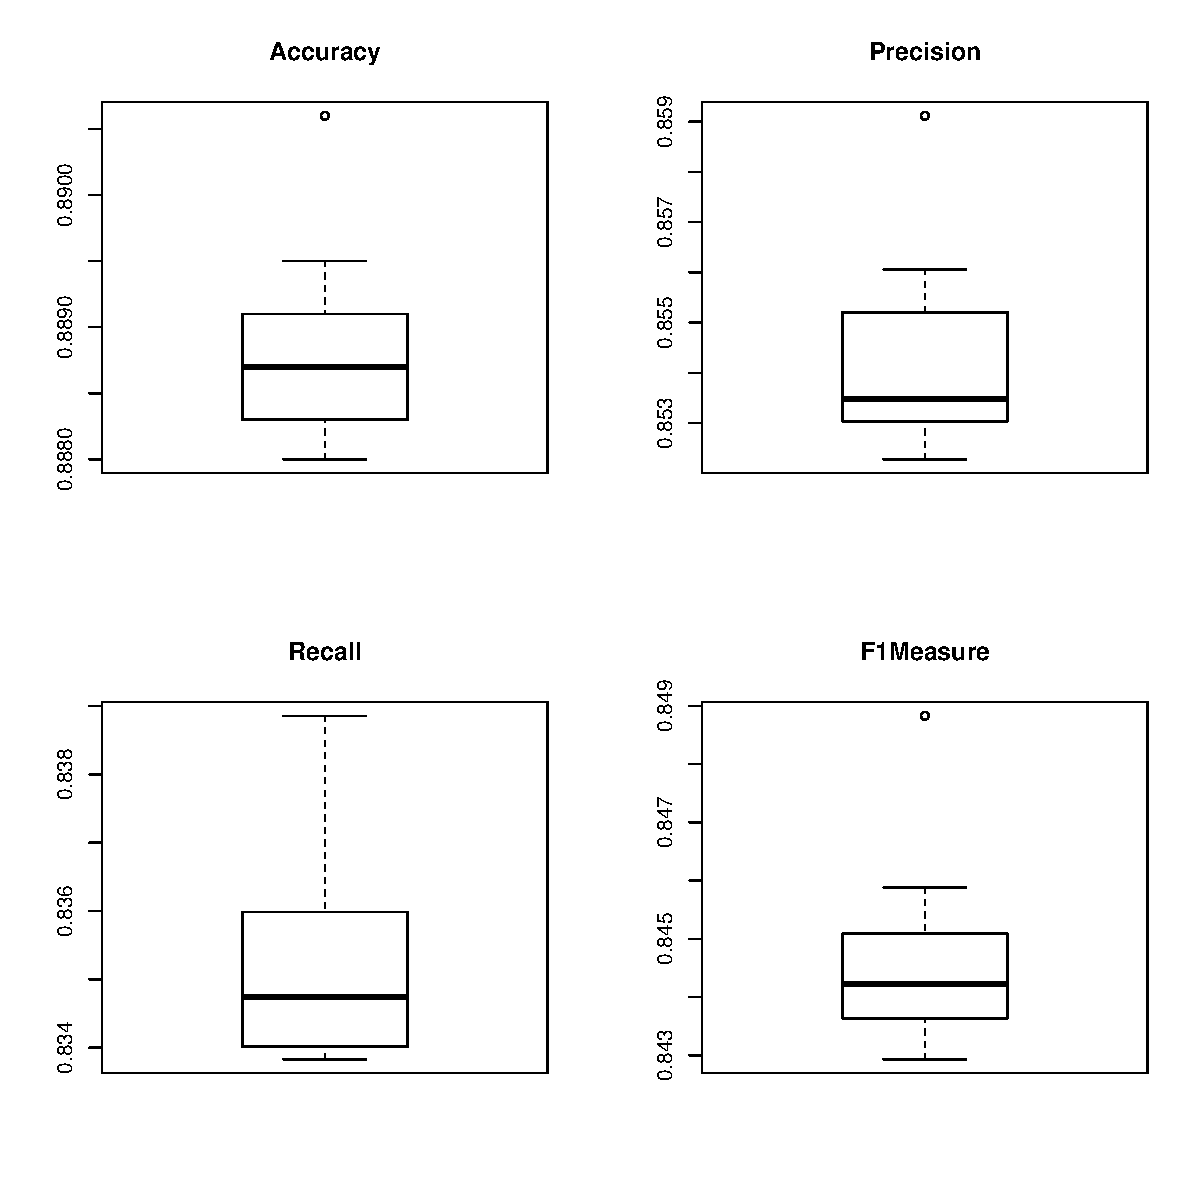
\includegraphics[width=0.7\linewidth]{images/paper_performance}
	\caption{Performance ottenute dalla rete proposta dal paper con evidenza completa dei nodi.}
	\label{fig:paperperformance}
\end{figure}
\begin{figure}
	\centering
	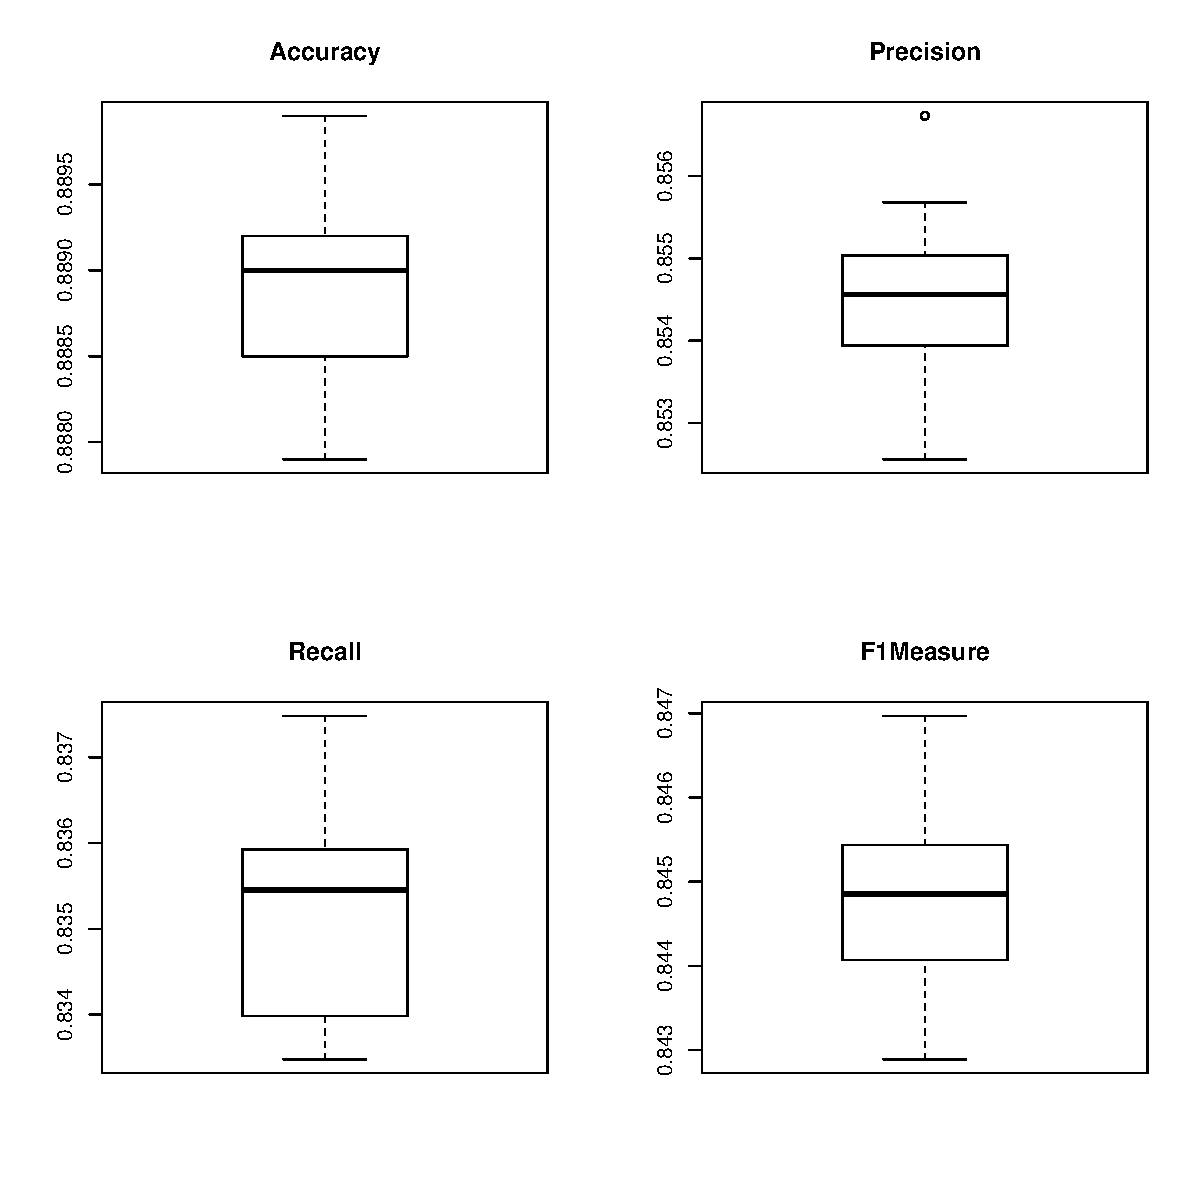
\includegraphics[width=0.7\linewidth]{images/induced_performance}
	\caption{Performance ottenute dalla rete appresa dal dataset con evidenza completa dei nodi.}
	\label{fig:inducedperformance}
\end{figure}
Questo è una conferma di come la struttura appresa dal dataset utilizzato sia valida e in grado di predire valori per il nodo \textit{Disease} in modo efficace; la presenza di un'unico arco in posizione differente non ha quindi impattato negativamente sulle performance predittive.

Analizzando più specificamente il dominio di applicazione, abbiamo deciso di ripetere le operazioni di inferenza del valore di \textit{Disease} fornendo non più un'evidenza completa delle variabili della rete, bensì fornendo solo di quei nodi che abbiamo ritenuto essere effettivamente osservabili dai medici, ovvero i dati del paziente e i risultati degli esami.\\
Le performance ottenute dalle due reti, riportate nelle Figure \ref{fig:paperperformancehalf} e \ref{fig:inducedperformancehalf}, sono, come ci aspettavamo, sensibilmente inferiori; ciononostante, le performance dei due modelli risultano nuovamente statisticamente non dissimili, avallando ulteriormente la tesi che la struttura appresa dai dati sia valida.\\
\begin{figure}
	\centering
	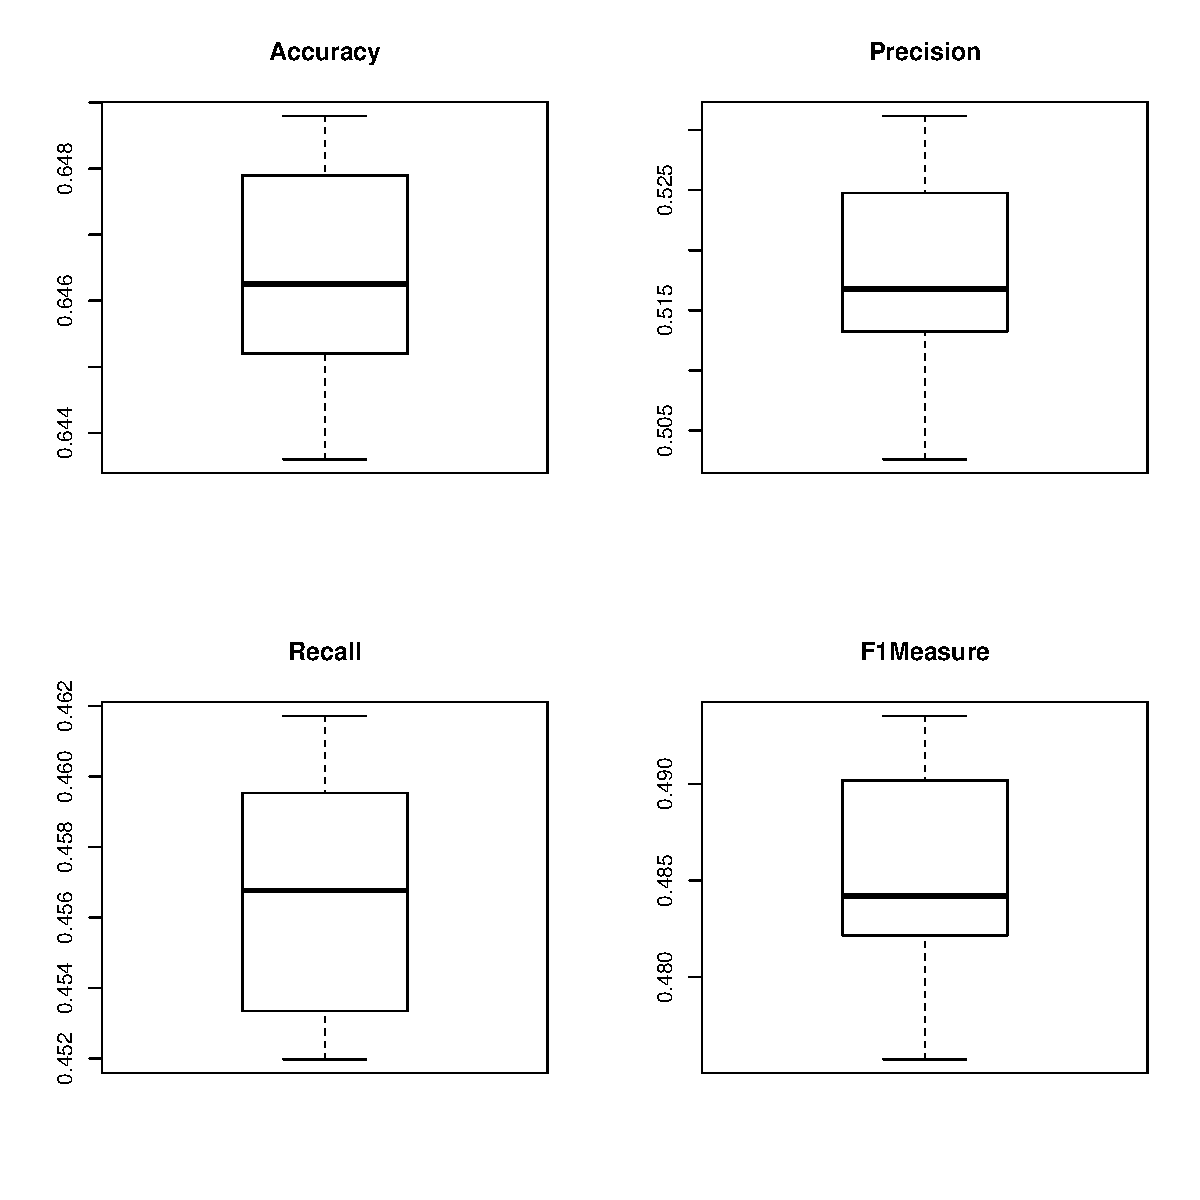
\includegraphics[width=0.7\linewidth]{images/paper_performance_half}
	\caption{Performance ottenute dalla rete proposta dal paper con solo esami e dati del paziente come evidenze.}
	\label{fig:paperperformancehalf}
\end{figure}
\begin{figure}
	\centering
	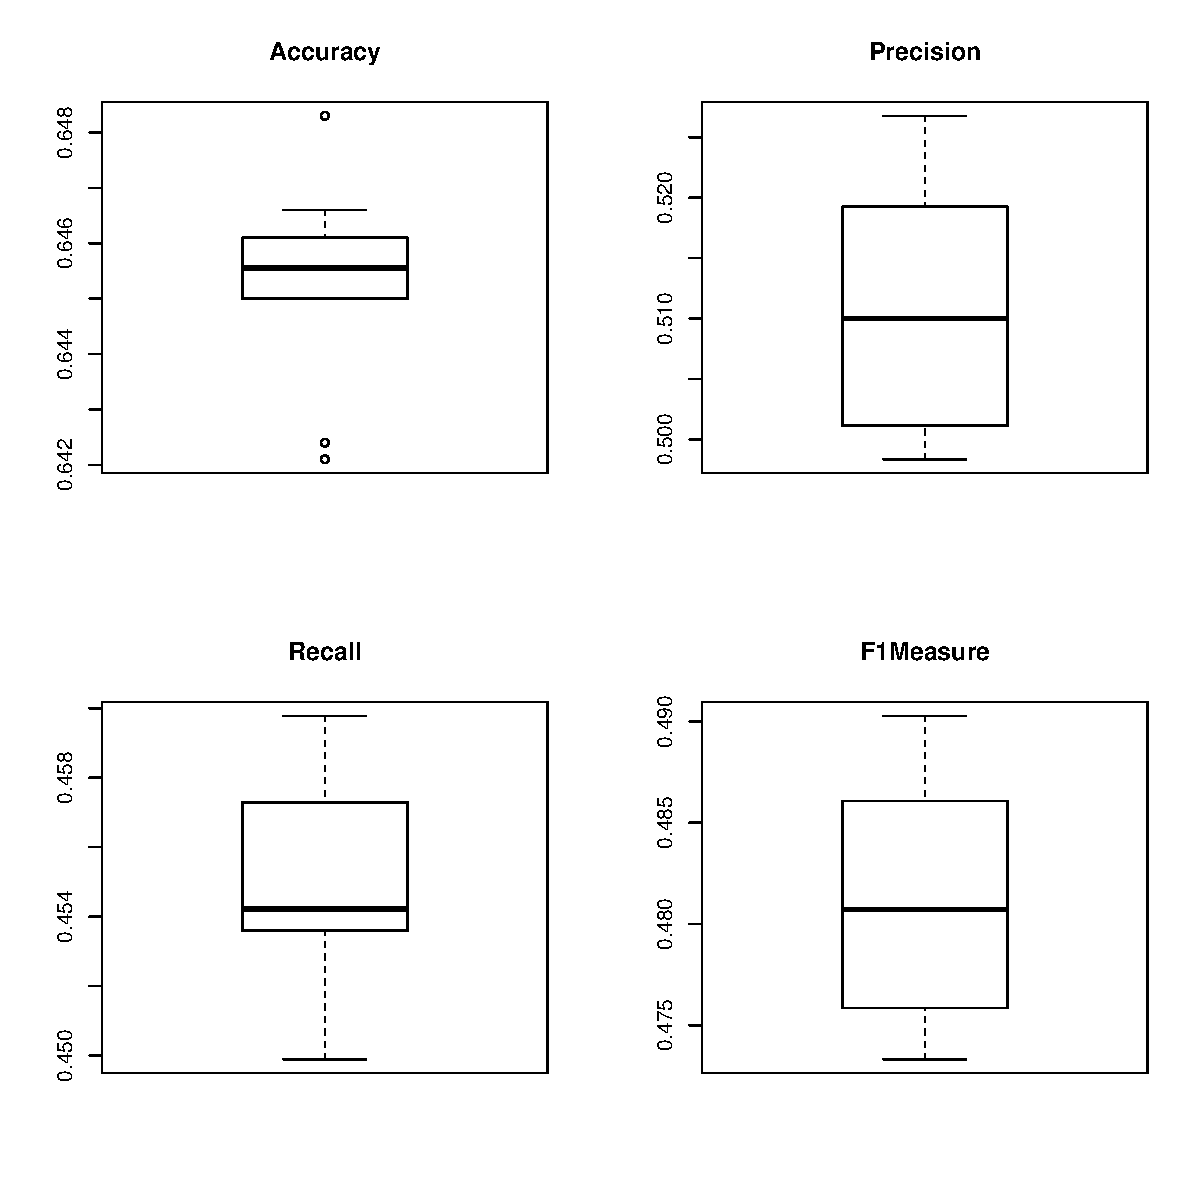
\includegraphics[width=0.7\linewidth]{images/induced_performance_half}
	\caption{Performance ottenute dalla rete appresa dal dataset con solo esami e dati del paziente come evidenze.}
	\label{fig:inducedperformancehalf}
\end{figure}

\section{Rete con struttura capovolta}
Seguendo un spunto proposto dal docente, abbiamo deciso di invertire il senso degli archi all'interno della rete proposta dal paper, capovolgendo di fatto le relazione di dipendenza causale nella rete. Dalla rappresentazione della rete ottenuta, riportata in Figura \ref{fig:reversedstructure}, abbiamo osservato come il numero medio di genitori per ogni nodo risulti essere molto maggiore rispetto alla rete proposta dal paper. In particolare, il nodo di maggiore interesse risulta avere ben sette genitori (contro il singolo genitore nella rete del paper), portando la dimensione della sua CPT a quasi $8000$ celle. 
\begin{figure}
	\centering
	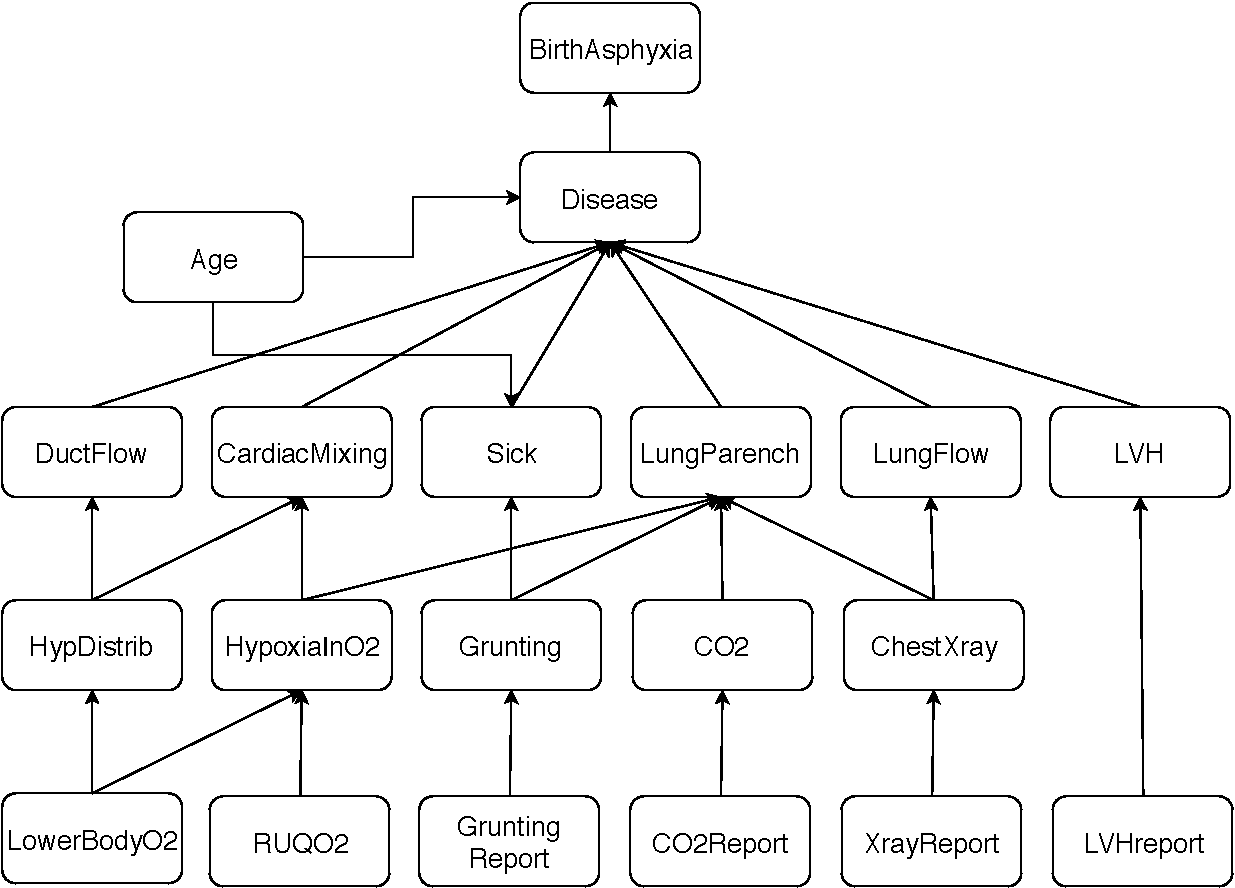
\includegraphics[width=1\linewidth]{images/reversed_structure}
	\caption{Struttura della rete proposta dal paper con la direzione degli archi invertita.}
	\label{fig:reversedstructure}
\end{figure}
Provando ad eseguire il processo di inferenza del nodo \textit{Disease}, otteniamo performance (riportate in Figura ) leggermente inferiori rispetto alla rete proposta dal paper; i test \textit{t-student} confermano che vi è una differenza statistica tra le medie di tutte le misure di performance analizzate. Analizzando le CPT ottenute nello specifico, appare come il modello sia andato in contro ad una creazione di tabelle molto specifiche, con probabilità associate a combinazioni di eventi pari a 0. Il drastico aumento del numero di genitori dei nodi ha quindi portato il modello a dover considerare una serie di combinazioni di eventi che in realtà non si propongono mai nel nostro dataset, assegnando a questi eventi probabilità pari a $0$. Il modello risulta quindi molto più complesso del dovuto, richiedendo di specificare un numero maggiore di parametri al fine del buon funzionamento dello stesso.
\begin{figure}
	\centering
	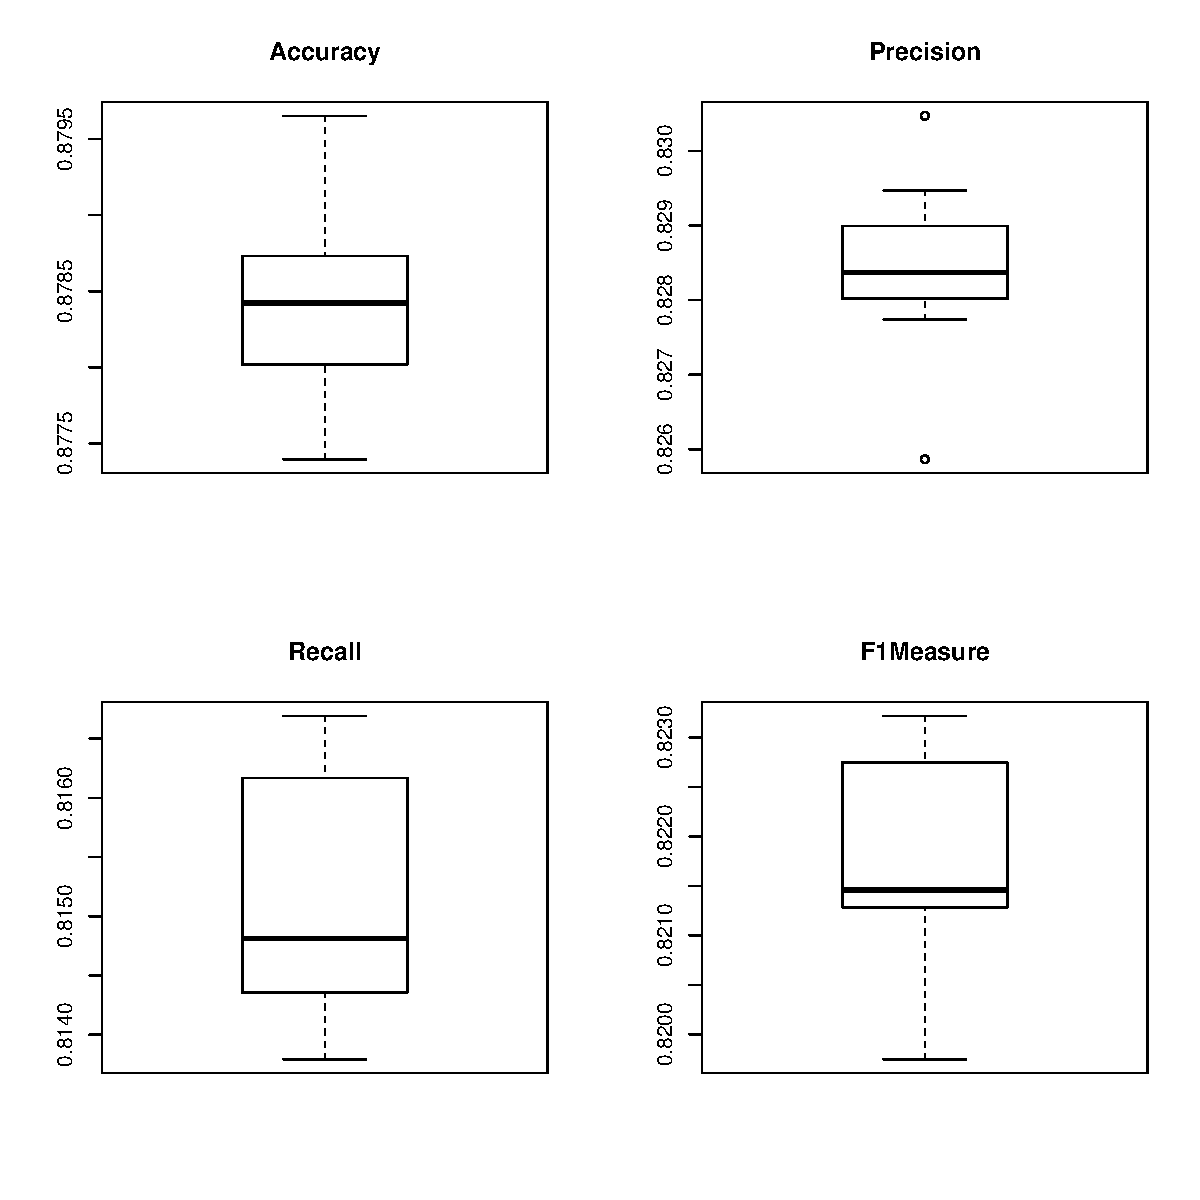
\includegraphics[width=0.7\linewidth]{images/reversed_performance}
	\caption{Performance ottenute dalla rete con archi invertiti dal paper con evidenza completa dei nodi.}
	\label{fig:reversedperformance}
\end{figure}


\section{D-separazione}
Nel nostro lavoro abbiamo cercato di individuare se vi fossero dei nodi all'interno della rete la cui evidenza garantisse l'indipendenza tra il nodo \textit{Disease} e un qualunque altro nodo. In un primo momento abbiamo cercato di individuare tutte le possibili combinazioni di evidenze che d-separassero una coppia di nodi, ma questo si è rivelato impraticabile, in quanto il processo produceva un file di testo di quasi 2Gb. Scartata l'opzione esaustiva, abbiamo deciso di produrre un'interfaccia che permetta di scegliere un qualunque sottoinsieme di evidenze, il nodo origine e il nodo destinazione e, tramite il calcolo della d-separazione, venisse restituito se i nodi scelti fossero o meno indipendenti dati l'evidenza. 
Analizzando la rete siamo giunti alla conclusione che il nodo \textit{Disease} risulti d-separato da alcuni esami date le condizioni che questi esami rilevano. Un esempio di ciò è la coppia di nodi \textit{Disease} e \textit{CO2} data l'evidenza del nodo \textit{LungParench}. Questo tipo di considerazione si rivela però essere un mero esercizio di stile, in quanto nel dominio di applicazione non è possibile stabilire se una condizione patologica sia presente o meno senza aver effettuato il relativo esame. Ne consegue quindi che nella rete non vi siano strutture di d-separazione utili a ridurre il numero di evidenze da rilevare al fine di stimare con accuratezza il valore del nodo \textit{Disease}.

\section{Fitting della rete e stima della CPT di \textit{Disease} data evidenza}
Avendo verificato, nella Sezione \ref{sec:performance} che la rete appresa dai dati risulta essere equivalente a quella proposta dal paper, abbiamo deciso di utilizzare quest'ultima per stimare le CPT dei nodi facenti parte della rete. Il risultato prodotto è riportato in Figura \ref{fig:paperfitted}. Ci siamo quindi chiesti come l'evidenza introdotta nella nostra rete potesse modificare la distribuzione di realizzazione del nodo \textit{Disease}, e se vi fossero quindi degli esami che fossero “migliori” di altri al fine di individuare quale fosse la malattia alla base della sindrome del \textit{BlueBaby}. Al fine di permettere al medico di introdurre le evidenze con un'interfaccia comoda ed intuitiva, è stata anche realizzata una demo che permette di inserire nella rete un insieme di evidenze a piacere e permette di ottenere la distribuzione di realizzazione del nodo \textit{Disease}.
\begin{figure}
	\centering
	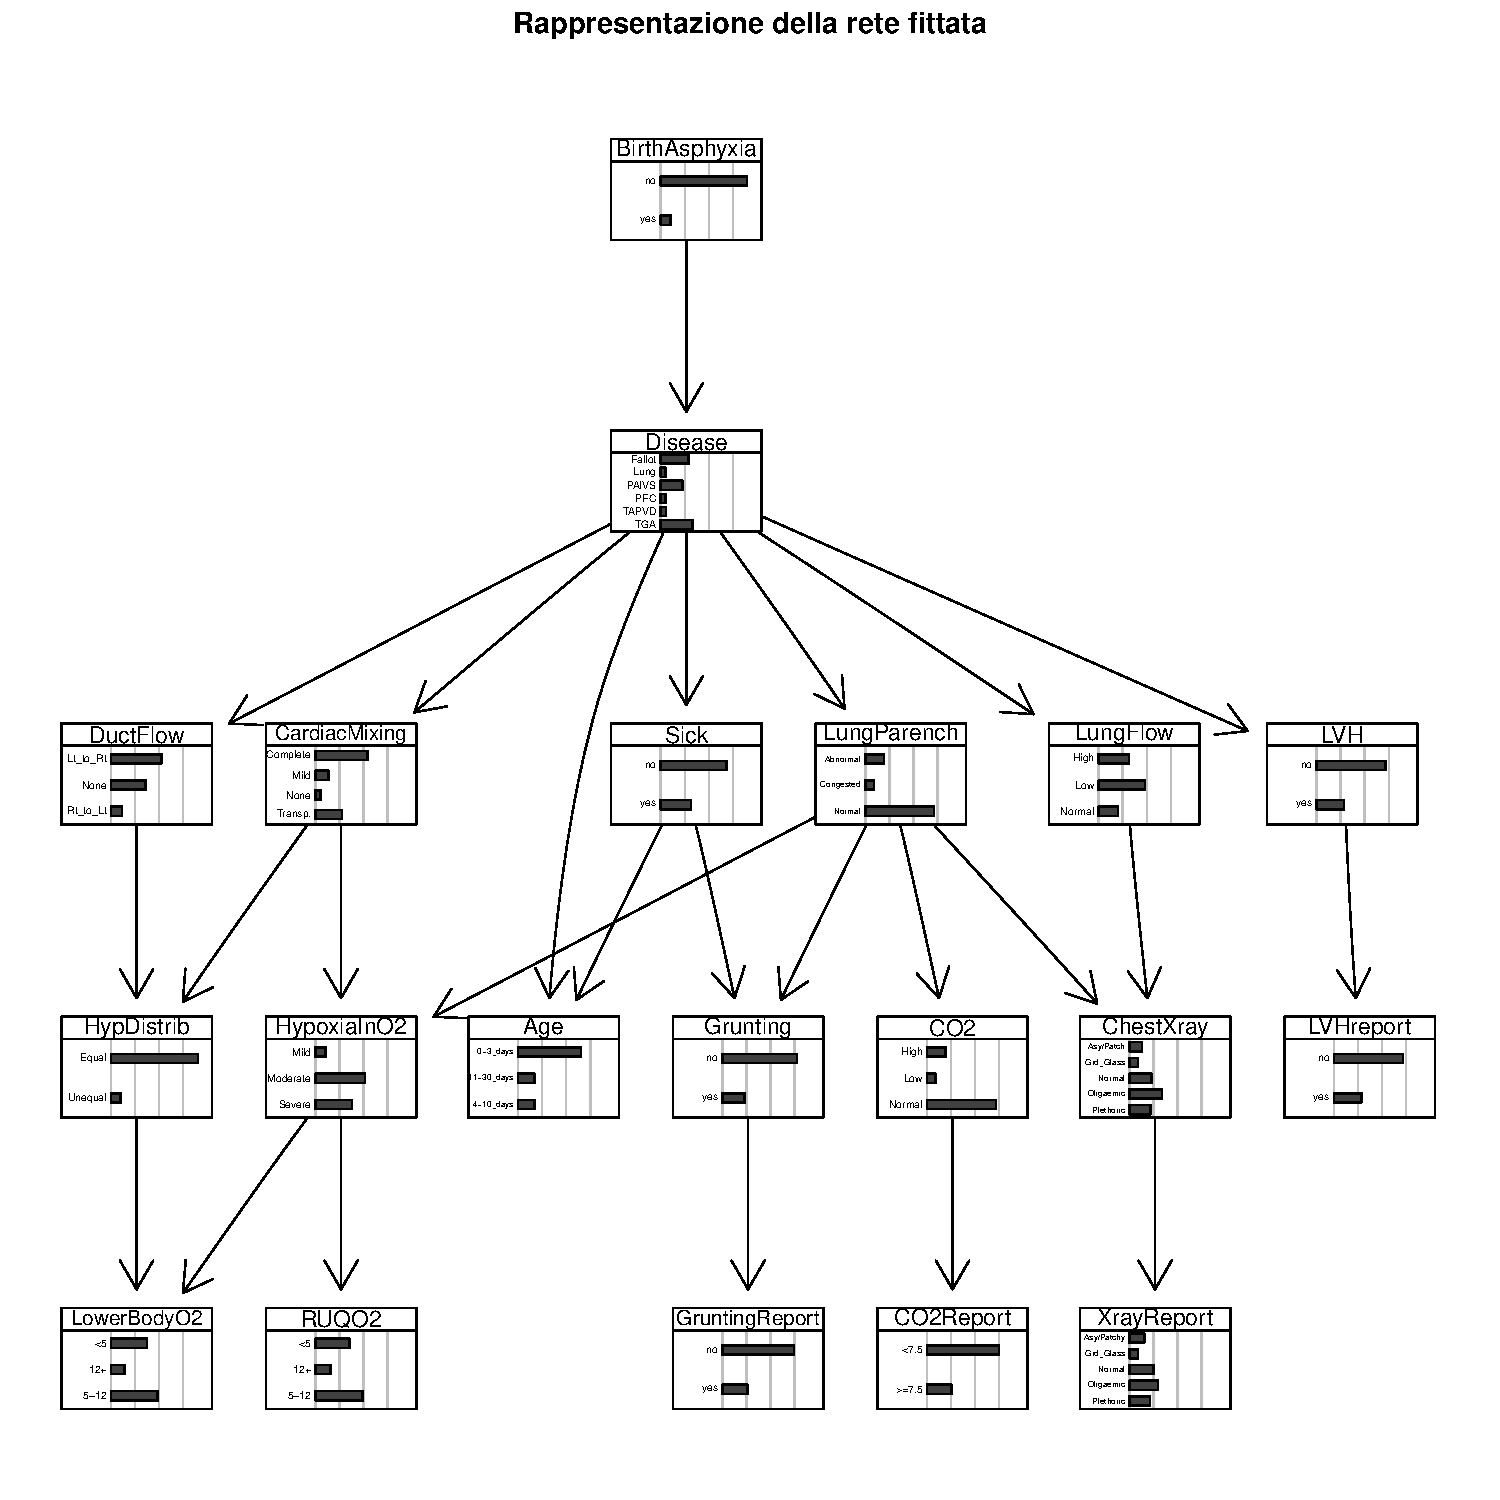
\includegraphics[width=1\linewidth]{images/paper_fitted}
	\caption{Rappresentazione della rete del paper al termine del processo di fitting con i dati contenuti nel dataset fornito.}
	\label{fig:paperfitted}
\end{figure}
Da questo tipo di analisi è emerso che alcuni valori dei nodi \textit{XrayReport} e \textit{LVHreport} modifichino la distribuzione di realizzazione di \textit{Disease} in modo significativo, portandolo ad assumere il valore di una particolare malattia oltre il $60\%$ delle volte. Se si avessero quindi a disposizione un limitato numero di esami, questi due permetterebbero di rilevale velocemente la possibile presenza di due delle 6 possibili patologie. Per quanto riguarda i restanti esami, non vi pare essere una chiara propensione per una malattia al variare del risultato di un singolo esame. Differente è il risultato se valutiamo più di un esame contemporaneamente: alcune combinazioni di osservazioni dei restanti esami permettono di ridurre drasticamente la probabilità di \textit{Disease} di avverarsi con alcuni valori, restringendo di fatto la ricerca a solo due o tre patologie possibili. 